\documentclass{ctexart}
%\CTEXsetup[name={Step ,},number={\arabic{chapter}}]{chapter}

\usepackage{amsmath}
%\usepackage{wallpaper}
\usepackage{xcolor}
%\usepackage{pgf, tikz}
\usepackage{multirow}
\usepackage{listings}
\usepackage{color}

\definecolor{keywordcolor}{rgb}{0.8,0.1,0.5}
\definecolor{webgreen}{rgb}{0,.5,0}

%\usepackage[paperwidth=185mm,paperheight=260mm,text={148mm,210mm},left=21mm,includehead,vmarginratio=1:1]{geometry}
%\usepackage[raggedright]{titlesec}
%\titleformat{\chapter}[display]{\Huge\bfseries}{Step \,\thechapter\,}{1em}{}

%\usepackage{fancyhdr}
%\pagestyle{fancy}
%\fancyhf{}
%\fancyhead[ER, OR]{\leftmark}
%\fancyhead[EL, OL]{《编译实习》实习报告}
%\fancyfoot[C]{\thepage}
%\renewcommand{\chaptermark}[1]{\markboth{\thechapter.\ #1}{}}


\lstset{language=C,
basicstyle=\footnotesize,
keywordstyle=\color{keywordcolor}\bfseries, %\underbar,
identifierstyle=,
commentstyle=\color{green} \textit,
stringstyle=\color{red} \ttfamily,
showstringspaces=false,
frame=single,
numbers=left,
numberstyle=\tiny \color{blue},
backgroundcolor=\color{white},
captionpos=b
}


\begin{document}

\title{%
\vspace{-30mm}\heiti\Huge NachOS Lab3 实习报告 \vspace{10mm}}
\author{%
\Large 史杨勍惟 
\\[10mm] 1200012741 信息科学技术学院}
\date{2015,03,30}

\maketitle

\newpage
\tableofcontents
\newpage

\section{总体概述}
这次的Lab主要内容是对于操作系统同步机制的理解,实现与应用。同步机制有多种实现方式,这次实验包括了三种主要的:
\begin{enumerate}
\item 信号量(Nachos已实现)
\item 互斥锁(Nachos未实现)
\item 条件变量(Nachos未实现)
\end{enumerate}
我们的任务是实现未实现的同步机制工具,并且在此基础上将它们应用到一些指定的同步机制上。

\section{任务完成列表}
\begin{table}[h]
\footnotesize
\begin{tabular}{|c|c|c|c|c|}\hline
\textbf{Exercise 1} & \textbf{Exercise 2} & \textbf{Exercise 3} & \textbf{Challenge 1} & \textbf{Challenge 2}\\\hline
Y & Y & Y & Y & N\\\hline

\end{tabular}

\end{table}
\section{完成情况}
\subsection*{Exercise 1}
\textbf{调研Linux中实现的同步机制}

Linux中为同步以及互斥机制提供了很多工具,主要有以下这些:
\begin{enumerate}
\item 原子操作:一种简单的实现互斥地方法,如果临界操作都是原子操作,那那些仅仅只有互斥关系的临界区相关进程就不会发生冲突。
\item 自旋锁:一个自旋锁只能被一个可执行线程持有,如果一个执行线程试图获得一个被已经持有的读写锁,那么这个线程就会一种忙等。 
\item 读写锁:读写锁是自旋锁的一种特殊形式,其设计是针对读者写者问题的,有了读写锁读者写者问题的同步机制就可以方便解决了。我们也可以为Nachos设计读写锁,这也是一个Challenge的内容,不过我没有实现。
\item 信号量:分二元和多元信号量。这个和Nachos中的信号量机制很像,也是Linux中唯一一个可以允许睡眠的锁。
\item 大内核锁:一个全局的自旋锁,主要是为了方便实现从Linux最初的SMP过渡到细粒度加锁机制。
\item 屏障:这也是我们这次Lab的一个Challenge所要实现的内容,主要是为了使得规范线程运行的顺序,屏障之后的内容会在屏障之前的内容执行完毕后执行。
\end{enumerate}

\subsection*{Exercise 2}
\textbf{仔细阅读代码,理解Nachos现有的同步机制}

正如概述中提到的,Nachos有三种同步机制的工具:信号量,锁和条件变量。

synch.h和synch.c定义了所有这三种同步工具的数据结构,以及内部的成员和方法。其中信号量是已经被实现了的。其数据结构为Semaphore,核心方法就是PV操作的P()和V(),而最重要的内部成员便是信号量的值value了。value由构造函数初始化,并且决定了P操作是否可以继续。如果value<0则P方法会被挂起到等待队列并进入休眠态,调用Sleep()唤起另一个线程。而V()操作则会激活等待队列中的第一个线程,调用ReadyToRun将其置为就绪态。

这个实现方法和上个学期操统课上所表示的基本一致,当然,PV操作作为原子操作,是要设置中断开关的。

这里我发现了一个问题,会不会在value++了以后,然后value>0后很多个线程同时进入P操作,这样这些线程就会同时跳过while了。不过后来发现他们被中断保护了,而且由于是跳过while循环所以不会进入休眠态,所以中断也不会在其他地方打开,这就保证了value--后其他线程还是会落入while循环。

\subsection*{Exercise 3}
\textbf{实现锁和条件变量}

在Nachos中,信号量,锁和条件变量并不是平行的。后者均可以基于前者实现。在这里,锁的实现使用了信号量,条件变量的实现使用了锁。

\subsubsection*{锁的实现}
代码如下:
\begin{lstlisting}
void Lock::Acquire() {
    IntStatus oldLevel = interrupt->SetLevel(IntOff);
    semaphore->P();
    holder = currentThread;
    (void) interrupt->SetLevel(oldLevel);
}
void Lock::Release() {
    IntStatus oldLevel = interrupt->SetLevel(IntOff);
    semaphore->V();
    holder = NULL;
    (void) interrupt->SetLevel(oldLevel);
}
bool Lock::isHeldByCurrentThread() {
    return holder == currentThread;
}
\end{lstlisting}
本质上Acquire和Release操作只是P和V的一个包装,只不过维护了holder成员并且添加了一些ASSERT断言,使得整个系统更加有秩序了一点。

\subsubsection*{条件变量的实现}
代码如下:
\begin{lstlisting}

void Condition::Wait(Lock* conditionLock) { 
    IntStatus oldLevel = interrupt->SetLevel(IntOff);
    ASSERT(conditionLock->isHeldByCurrentThread());
    DEBUG('t', "in waiting\n");
    if(waitList->IsEmpty()) {
        lock = conditionLock;
    }

    waitList->Append(currentThread);
    conditionLock->Release();
    currentThread->Sleep();
    conditionLock->Acquire();
    (void) interrupt->SetLevel(oldLevel);
}

void Condition::Signal(Lock* conditionLock) { 
    IntStatus oldLevel = interrupt->SetLevel(IntOff);
    DEBUG('t', "in signaling\n");
    ASSERT(conditionLock->isHeldByCurrentThread());
    if(!waitList->IsEmpty()) {
        Thread* nextThread = (Thread *) waitList->Remove();
        scheduler->ReadyToRun(nextThread);
    }
    (void) interrupt->SetLevel(oldLevel);
}
void Condition::Broadcast(Lock* conditionLock) { }

\end{lstlisting}
Condition的实现是参考信号量的实现完成的。其中对条件锁进行了维护。而waitList和信号量中的queue是完全一样的作用。

\subsection*{Exercise 4}
\textbf{实现同步互斥实例}

我选择的是生产者消费者问题,选用了信号量和条件变量两种实现方式。其中ThreadTest4函数是共用的,如下:
\begin{lstlisting}
void ThreadTest4() {
    Thread *t1 = new Thread("producer thread");
    Thread *t2 = new Thread("consumer thread");
    t2->Fork(Consumer, 2);
    t1->Fork(Producer, 1);
}
\end{lstlisting}

\subsubsection*{信号量实现}
信号量的实现方式基本就是经典的生产者消费者的实现方式,这里我就不详述了,直接用如下代码就可以看出规则了。
\begin{lstlisting}
void Producer(int tid) {
    for(int i = 0; i < 10; ++i) {

        pLock->P();
        mutex->P();
        printf("producing %d\n", i);
        mutex->V();
        cLock->V();
    }
}

void Consumer(int tid) {
    for(int i = 0; i < 10; ++i) {
        cLock->P();
        mutex->P();
        printf("consuming %d\n", i);
        mutex->V();
        pLock->V();
    }
}
\end{lstlisting}
其中信号量的初始化如下:
\begin{lstlisting}
Semaphore * pLock = new Semaphore("PLOCK", BUFFERSIZE);
Semaphore * cLock = new Semaphore("CLOCK", 0);
Semaphore * mutex = new Semaphore("MUTEX", 1);
\end{lstlisting}
最后结果如下:
\begin{figure}[h!]
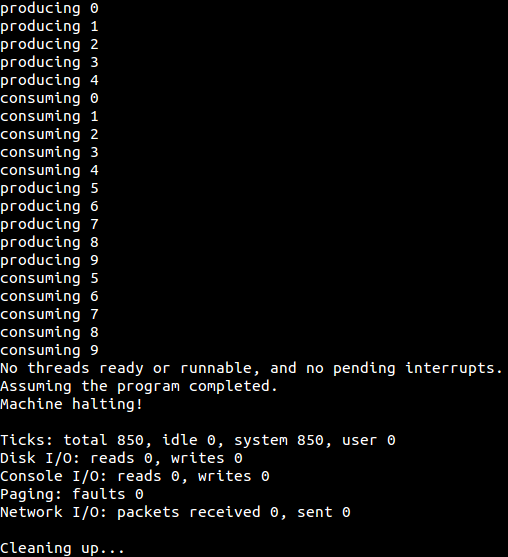
\includegraphics[width=2.5in]{e30.png}
\end{figure}

\subsubsection*{条件变量实现}
条件变量的实现我纠结了很长的时间,毕竟以前基本这种同步问题都是用PV操作来实现的,很少使用过条件变量。而且条件变量需要和锁配合使用,所以还是有些麻烦的。在这个过程中我也到网上寻找了一些用条件变量实现生产者消费者问题的方法,最终整合并修改后得到了如下版本的代码。

\begin{lstlisting}
void Producer(int tid) {
    for(int i = 0; i < 10; ++i) {
        lmutex->Acquire();
        while(buffer == BUFFERSIZE) {
            lpLock->Acquire();
            lmutex->Release();
            lpCond->Wait(lpLock);
            lmutex->Acquire();
            lpLock->Release();
        }
        buffer++;
        printf("producing! %d products left\n", buffer);
        lcLock->Acquire();
        lcCond->Signal(lcLock);
        lcLock->Release();
        lmutex->Release();
        currentThread->Yield();
    }
}

void Consumer(int tid) {
    for(int i = 0; i < 10; ++i) {
        lmutex->Acquire();
        while(buffer == 0) {
            lcLock->Acquire();
            lmutex->Release();
            lcCond->Wait(lcLock);
            lmutex->Acquire();
            lcLock->Release();
        }
        printf("consuming! %d products left\n", buffer);
        buffer--;
        lpLock->Acquire();
        lpCond->Signal(lpLock);
        lpLock->Release();
        lmutex->Release();
        currentThread->Yield();
    }
}
\end{lstlisting}
其中变量初始化如下:
\begin{lstlisting}
int buffer = 0;
Lock * lmutex = new Lock("MUTEX");
Lock * lcLock = new Lock("CLOCK");
Lock * lpLock = new Lock("PLOCK");
Condition * lcCond = new Condition("CCOND");
Condition * lpCond = new Condition("PCOND");
\end{lstlisting}
最后的运行结果如下:
\begin{figure}[h!]
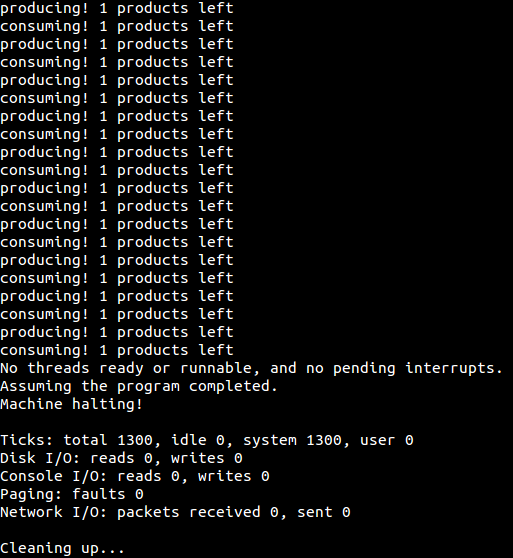
\includegraphics[width=2.5in]{e311.png}
\end{figure}
然后我对序列顺序做了一下修改,把Producer和Consumer中的Yield去除了,得到了如下的结果:
\begin{figure}[h!]
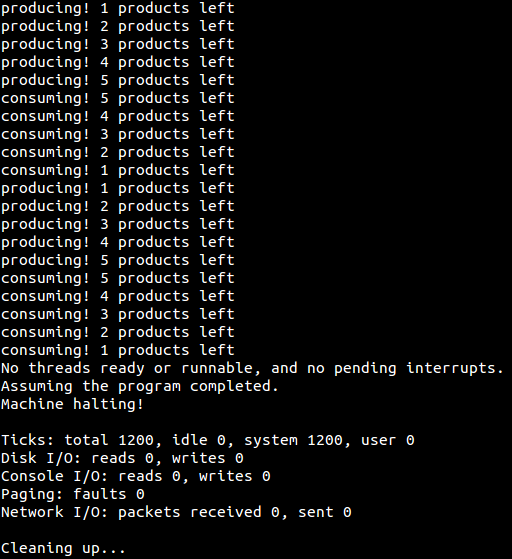
\includegraphics[width=2.5in]{e310.png}
\end{figure}

这两个结果是符合逻辑的,一个是一个一个接着来,另一个是消费者和生产者一起来。

\subsection*{Challenge 1}
\textbf{实现Barrier}
正如Exercise 1中所叙述的,Barrier的主要功能便是规范线程的执行顺序,Barrier之后的代码要在所有线程(有barrier的线程)运行到barrier之后才可执行。这里我创建了一个Barrier数据结构,代码如下。
\begin{lstlisting}
class Barrier {
    public:         
        Semaphore  * semaphore;
        int count;
        vector<Semaphore *> semList;
        Barrier(int _count);
        ~Barrier();        
        void setBarrier(int i);
        void initBarrier();
};

void barrierFunc(int arg) {
   Barrier * barrier = (Barrier*) arg;
   barrier->semaphore->P();
   for(int i = 0; i < barrier->semList.size(); ++i) {
       barrier->semList[i]->V();
   }
}

void Barrier::initBarrier() {   
    DEBUG('t', "INIT BARRIER\n");
    for(int i = 0; i < count; ++i) {
        Semaphore * bsemaphore = new Semaphore("THREADSEM", 0);
        DEBUG('t', "%d thread in barrier init\n", bsemaphore);
        semList.push_back(bsemaphore);
    }
    Thread * barrierThread = new Thread("barrier"); 
    barrierThread->Fork(barrierFunc, int(this));
}

void Barrier::setBarrier(int i) {
    DEBUG('t', "in set barrier\n");
    semaphore->V();
    DEBUG('t', "%d %d \n", i, semList[i]);
    semList[i]->P();
    DEBUG('t', "in set barrier 3\n");
}
\end{lstlisting}

Barrier的初始化需要传递一个参数count,这个参数表示了有多少个线程需要设置Barrier,与此同时初始化一个负值信号量,并初始化了一个信号量数组。在init函数中,Fork出了一个新的线程,这个线程会在Barrier信号量回到正值了(表示所有线程到达了Barrier)以后对数组的每个信号量进行V操作。

在线程中通过在指定位置调用setBarrier函数设置Barrier,在setBarrier中,这个线程会对Barrier信号量进行一次V操作,并且停留在信号量数组的一个信号量上。只有当所有线程都到了Barrier后,Fork出的线程才会释放数组中的每个信号量,使得线程可以继续执行。

测试方法如下:
\begin{lstlisting}
Barrier * barrier = new Barrier(3);

void bthread(int arg) {
   printf("before barrier\n");
   barrier->setBarrier(arg);
   printf("after barrier\n");
}

void ThreadTest5() {
    Thread *t0 = new Thread("t50");
    Thread *t1 = new Thread("t51");
    Thread *t2 = new Thread("t52");
    barrier->initBarrier();
    t0->Fork(bthread, 0);
    t1->Fork(bthread, 1);
    t2->Fork(bthread, 2);
}
\end{lstlisting}
结果如下:

\begin{figure}[h!]
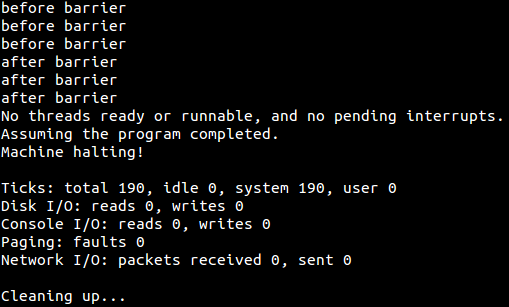
\includegraphics[width=2.5in]{e32.png}
\end{figure}

这个结果是正确的。

\section{遇到的困难以及解决办法}
\subsection*{条件变量的理解与使用}
条件变量对我来说是一个不算太熟悉的概念,虽然上个学期说的管程和条件变量有着密切的关系,但是我有没有透彻理解。这次条件变量的使用我也参阅了网上的内容。其实我现在看来条件变量只是信号量的一种拓展,并且把条件锁纳入其中了,所以看上去也并没有特别复杂。
\subsection*{Barrier机制的实现}
Barrier机制是一个比较奇特的机制,不过对于他怎么样实现我还是斟酌了许久。每一个机制的实现都有两部分,一个事内部实现,还有一个是外部调用方法。我的第一个版本的Barrier几乎全都使用了外部调用,把大部分的内容放在了threadtest中。但是出于系统设计的思想,应该尽可能把内容放到内部实现中,于是我创造了一个类,并且把大部分方法封装到类中实现,这也是C++的一个强大的应用点。

\section{收获与感想}

这次Lab的内容不多,代码量不算很大,涉及的文件也不算很多。但是主要的难度在于设计上,尤其是机制的设计和应用的设计,我觉得这两方面也是我目前还不算很强的地方。
通过这次Lab,我更深层次地理解了同步机制,通过自己实现我也对里面的细节有了更多的认识。与此同时,通过调研和Challenge我也了解了更多的同步机制工具,如Barrier。
我进一步认识了设计一个系统所需要考虑的要素,比如如何对机制进行封装,面向对象地实现。

\section{意见与建议}
我认为助教和老师应该在课上多讲一些内容,而不是把主要让同学发言。

\section{参考资料}
\begin{itemize}
\item 《现代操作系统》
\item 《Linux内核设计与实现》
\item  http://blog.sina.com.cn/s/blog728fa8670101erhb.html
\end{itemize}

\end{document}